\documentclass{article}
\usepackage[T1]{fontenc}
\usepackage{lmodern}
\usepackage{graphicx}
\usepackage{amsmath,amssymb}
\usepackage[a4paper,margin=2cm]{geometry}
\usepackage[absolute,overlay]{textpos}
\setlength{\TPHorizModule}{1mm}
\setlength{\TPVertModule}{1mm}
\usepackage[indonesian]{babel}
\usepackage{hyperref}
\setlength{\emergencystretch}{2em}
% unit: Halaman 12

\begin{document}

% === Halaman 12 (python/native) ===

12

3.

Chosen-plaintext attack 


Kriptanalis dapat memilih plainteks sesuka hati untuk dienkripsikan, yaitu 

plainteks-plainteks yang lebih mengarahkan penemuan kunci, lalu mengirim 

plainteks ke sistem enkripsi.  Asumsi: Penyerang memiliki akses ke sistem enkripsi

Diberikan:   P1, C1 = Ek(P1), P2, C2 = Ek(P2), …, Pi,  Ci = Ek(Pi)  

di mana kriptanalis dapat memilih diantara P1, P2, …, Pi 

             Deduksi:  k untuk mendapatkan Pi+1 dari Ci+1 = Ek(Pi+1).

% deskripsi: gambar native xref 122
\noindent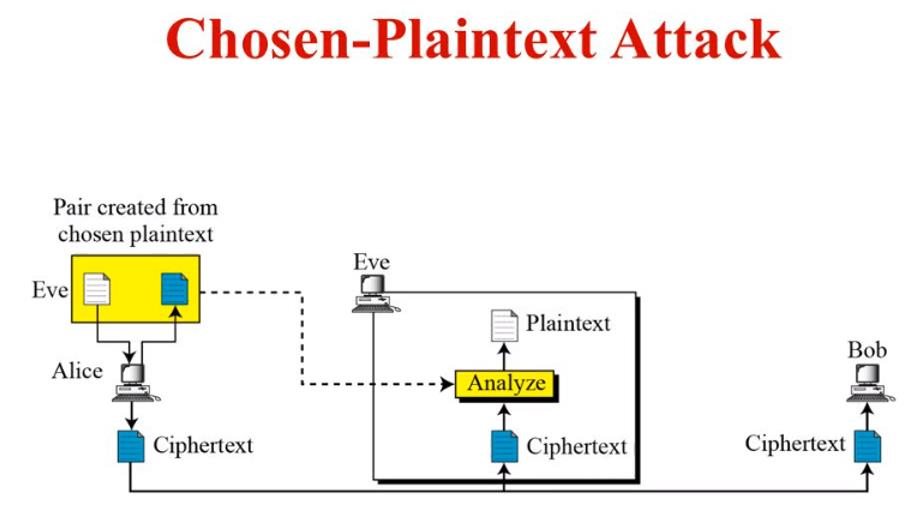
\includegraphics[width=0.85\textwidth]{../../images/python/page_012_img_01.jpeg}

\end{document}
